% Name: Stack and queue
% Description: A stack that pushes and pops at its top, beside a queue that adds at its back and removes from its front.
% Tags: stack, queue, LIFO, FIFO

\usetikzlibrary{arrows.meta}

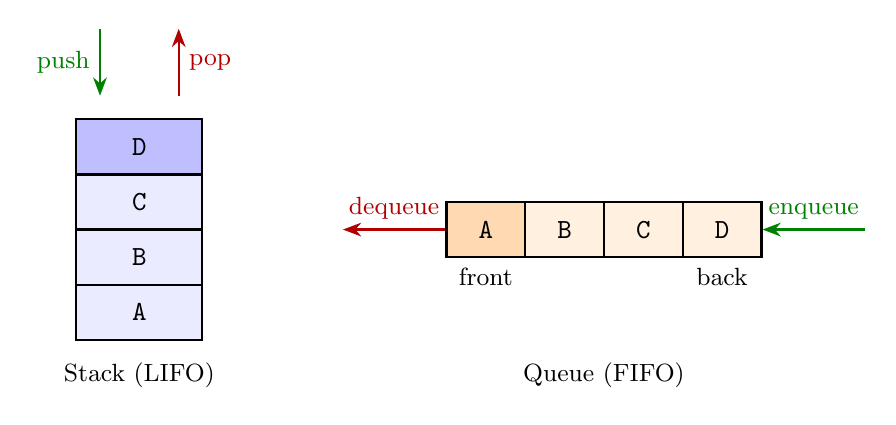
\begin{tikzpicture}[>={Stealth}, cell/.style={draw, thick, minimum width=16mm, minimum height=7mm, font=\ttfamily}, every label/.style={font=\small}]
  % The stack: last in, first out.
  \foreach \v [count=\i from 0] in {A, B, C, D}
    \node[cell, fill=blue!8] (s\i) at (0,\i*0.7) {\v};
  \node[cell, fill=blue!25] at (s3) {D};
  \draw[->, thick, green!50!black] (-0.5,3.6) -- node[left, font=\small] {push} (-0.5,2.75);
  \draw[->, thick, red!70!black] (0.5,2.75) -- node[right, font=\small] {pop} (0.5,3.6);
  \node[font=\small] at (0,-0.8) {Stack (LIFO)};
  % The queue: first in, first out.
  \foreach \v [count=\i from 0] in {A, B, C, D}
    \node[cell, minimum width=10mm, fill=orange!12] (q\i) at (4.4+\i*1,1.05) {\v};
  \node[cell, minimum width=10mm, fill=orange!30] at (q0) {A};
  \draw[->, thick, red!70!black] (q0.west) -- ++(-1.3,0) node[midway, above, font=\small] {dequeue};
  \draw[<-, thick, green!50!black] (q3.east) -- ++(1.3,0) node[midway, above, font=\small] {enqueue};
  \node[font=\small] at (q0.south) [below] {front};
  \node[font=\small] at (q3.south) [below] {back};
  \node[font=\small] at (5.9,-0.8) {Queue (FIFO)};
\end{tikzpicture}
